\subsubsection{概要}
むぎまるチームは1章で述べた目標のために, 
膨張リセット\cite{ueda2004iros}による破綻の修復と
2D LiDARのスキャンデータを用いる
Monte Carlo localization(MCL)\cite{fox1999etal}が
ROS 2で実装されたemcl2\_ros2\cite{emcl2_ros2}を使用した. 
スキャンデータは, 3D LiDARの点群データを高さ方向で圧縮し, 
2次元のデータとすることで作成した. 
スキャンデータの取得に2D LiDARではなく3D LiDARを用いた意図は, 
2D LiDARでは検出不可能な高さの障害物も検出可能にするためである. 
次項ではシステム構成を詳細に説明する. 

\subsubsection{システム構成}
むぎまるチームのシステム構成について説明する. 
ロボットに搭載した計算機, センサ, アクチュエータの接続の関係及び
計算機で実行するROS 2ノードの概要を表したものを
図\ref{fig:mugimaru_system}に示す. 

Raspberry Piには, IMUとエンコーダ, 車輪駆動用の
モータを接続した. 
実行するノードとしては, IMU用のROS 2ドライバノード(rt\_usb\_9axisimu\_driver)と, 
オドメトリの出力とモータの制御を実施するノード(raspimouse)がある. 
後者のノードでは, エンコーダの値と
前者のノードで配信されたIMUの情報からロボットのオドメトリを計算し, 
トピックとして配信する. 
モータの制御は, 外部のノードからトピックとして受信した
ロボットの速度指令をもとに実行する. 

PCには, 3D LiDARとRaspberry Piを接続した. 
実行するノードとしては, 3D LiDARに関係するノードが2つ, 
ロボットの自己位置推定とナビゲーションを実行するノードがある. 
3D LiDARに関係するノードとしては, Livox用のROS 2ドライバノード(livox\_lidar\_publisher)と, 
3D LiDARからの3次元点群を2次元に圧縮し, 
トピックとして配信するノード(pointcloud\_to\_laserscan)がある. 
自己位置推定には, 前項のとおりemcl2\_ros2を使用した. 
図中には, ノード名として「emcl2」と表している. 
このパッケージでは, 走行する環境の地図が必要となり, 
その作成にはROS 2標準のSLAMパッケージである
slam\_toolbox\cite{slam_toolbox}を使用した. 
ナビゲーションにはROS 2で標準的なロボットのナビゲーションパッケージである
navigation2\cite{nav2}を使用した. 
図中には, このパッケージに内包されるノードをまとめて「navigation2」と表している. 

\begin{figure}[h]
  \begin{center}
    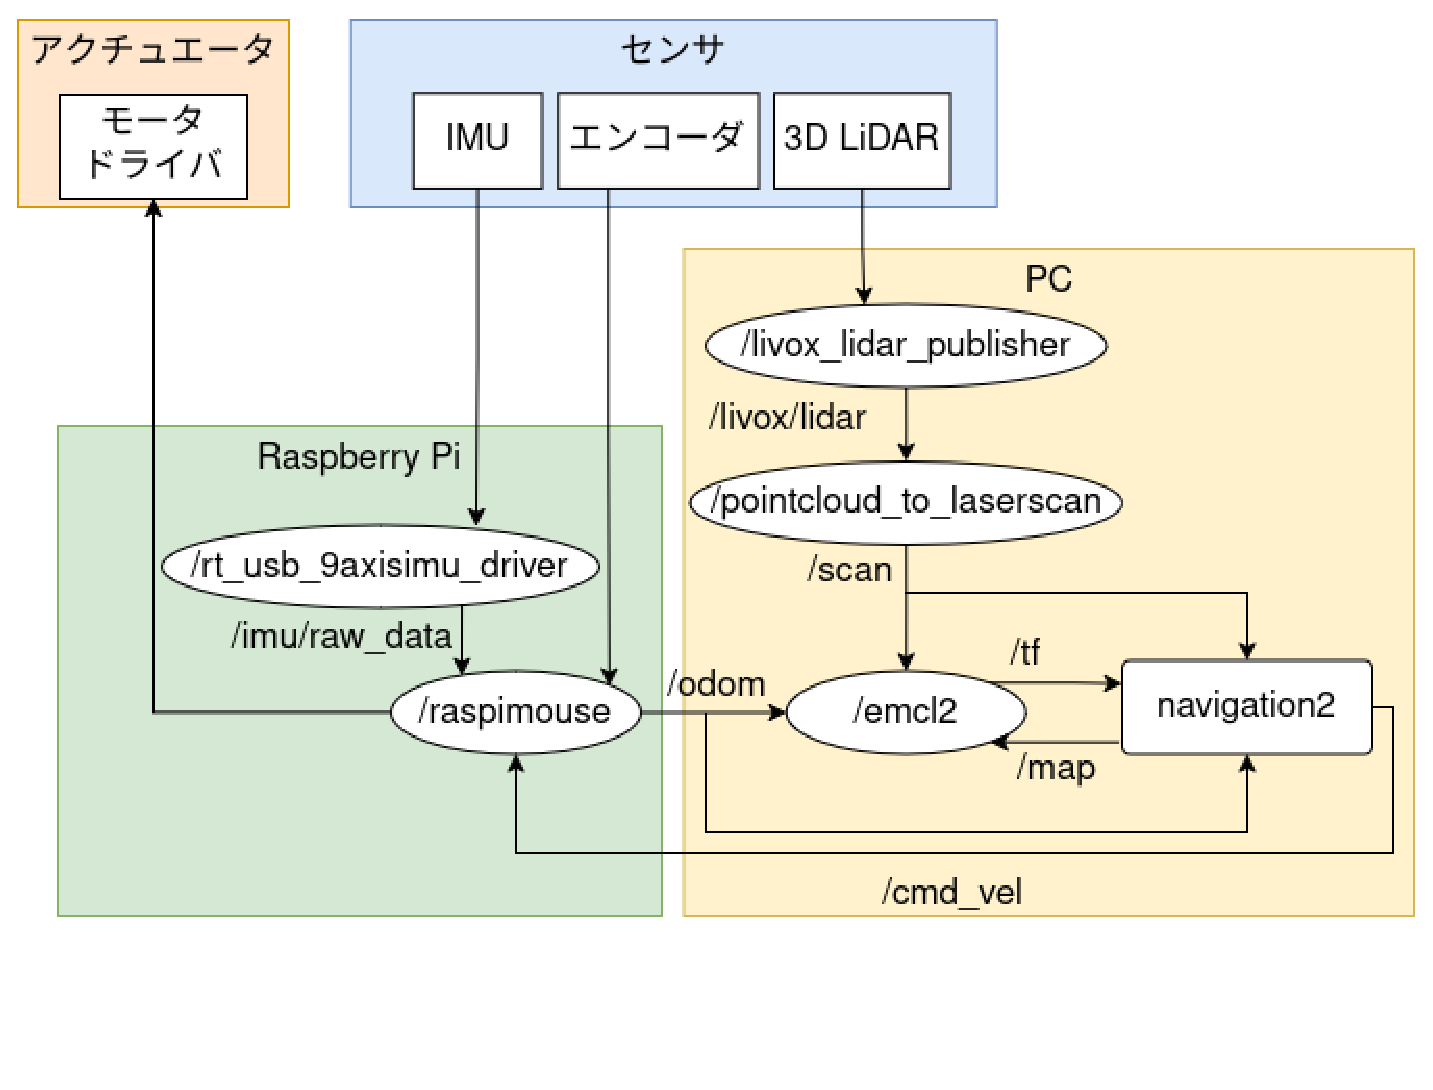
\includegraphics[width=1.0\linewidth]{figs/mugimaru_system_2024.eps}
    \caption{むぎまるチームのシステム構成}
    \label{fig:mugimaru_system}
  \end{center}
\end{figure}

